\documentclass{article}

\usepackage{arxiv}

\usepackage[utf8]{inputenc}
\usepackage[T1]{fontenc}
\usepackage{url}
\usepackage{booktabs}
\usepackage{amsfonts}
\usepackage{nicefrac}
\usepackage{microtype}
\usepackage{graphicx}
\usepackage[font=small,labelfont=bf]{caption}
\usepackage{cite}
\usepackage{pdflscape}
\usepackage{listings}
\usepackage{outlines}

\title{Logs lineage and tiered segments in Apache Kafka}

\begin{document}

\section{Disclaimer}
This document is a work-in-progress and is likely to be loaded with inaccuracies. To be taken with caution.

\section{Objectives}
The purpose of this document is to describe how remote log segments (offloaded to a tiered storage and not available in brokers log directories) are handled to guarantee an access to data agnostic of the storage tier.


\subsection{Data Uniform Access}

One \textbf{possible} functional behaviour could be to provide the same data to consumers regardless of the origin \footnote{i.e., informally, whether the data is stored and read from either the first (local) or second (remote) tier.} of these data. This \textit{uniformity} requires to reproduce the current behaviour of Apache Kafka for which log segments are always accessed locally.

If \textit{data uniformity} is chosen, the current specifications under divergence of log lineage should be preserved, and no discrepancy should be introduced in the data a consumer would expect to find with or without tiered storage.

\subsection{Notations}
Consider a topic-partition. In this document, we will note $S_i^r$ the i-th segment of a replica $r \in AR$ and $[BO_i^r..EO_i^r]$ the range of offsets of $S_i^r$ from the base offset $BO_i^r$ to the end offset $EO_i^r$. The log end offset at epoch $k$ is referred to as $LEO_k$\footnote{$LEO[LG_K]$ in figures.}.

\section{Preservation of local replica lineage in case of diverging replicas partially or totally tiered}

One consequence of unclean leader election is a possible divergence of log lineages which can happen when leadership of a topic-partition moves to an out-of-sync replica. It is possible that a log segment which is offloaded (uploaded) to a tiered storage presents offset overlap or contains duplicated and/or divergent records with already tiered log segments

Let us consider the following simplified example. A topic-partition is made of two replicas 1 and 2 on a cluster with tiered storage available and unclean leader election enabled. 

\begin{outline}[enumerate]
	\1 At $t_1$, replica 1 is the leader and replica 2 is out of the ISR set. The segment $S_i^1$ has been rolled over, and $S_{i+1}^1$ is the active segment or replica 1. Since the ISR is reduced to the leader replica, the leader high watermark can progress to the log end offset $LEO_k$. Assume there is no transactional records, so that the log stable offset corresponds to the leader high watermark, so that segment $S_i^1$ is eligible for tiering. Assume the leader 1 offloads successfully $S_i^1$ which is mapped to the unique ID $u_k$. Assume that afterwards, that segment is locally deleted to honor the configured log's retention policy.
	\1  At $t_2$, replica 1 becomes offline and replica 2, then only live replica of the topic-partition, is elected as the leader. Leader generation is incremented from $k$ to $k + 1$.
	\1  At $t_3$, replica 1 is back online and becomes a follower of replica 2. It truncates its local log to $LEO_{k+1}$, which is outside of the range of offsets covered by the local segments. However, assume that $LEO_{k+1} \in [BO_i^1..EO_i^1]$ which is a range of offsets covered in the tiered storage. Also, note that by construction of this example, the leader epoch of replica 1 before becoming follower is $k$. The follower 1 then decides to onload the segment with the key $u_k$. Truncation to $LEO_{k+1}$ then occurs as would have initially been for a local segment. In this example, this results in few diverging records, which were produced to $S_j^2$ but not replicated to $S(u_k)$.
	\1 At $t_4$, replica 2 ingested enough records for the segment $S_j^2$ to be rolled-over and tiered, assuming the necessary conditions are met. This results in two segments in the tiered storage with duplicated and divergent records.
\end{outline}

The principle guiding this proposal is to offer a uniform data access to consumers. This means the behaviour needs to be exactly identical whether the $S_i^1$ is remote or local.

\begin{center}
	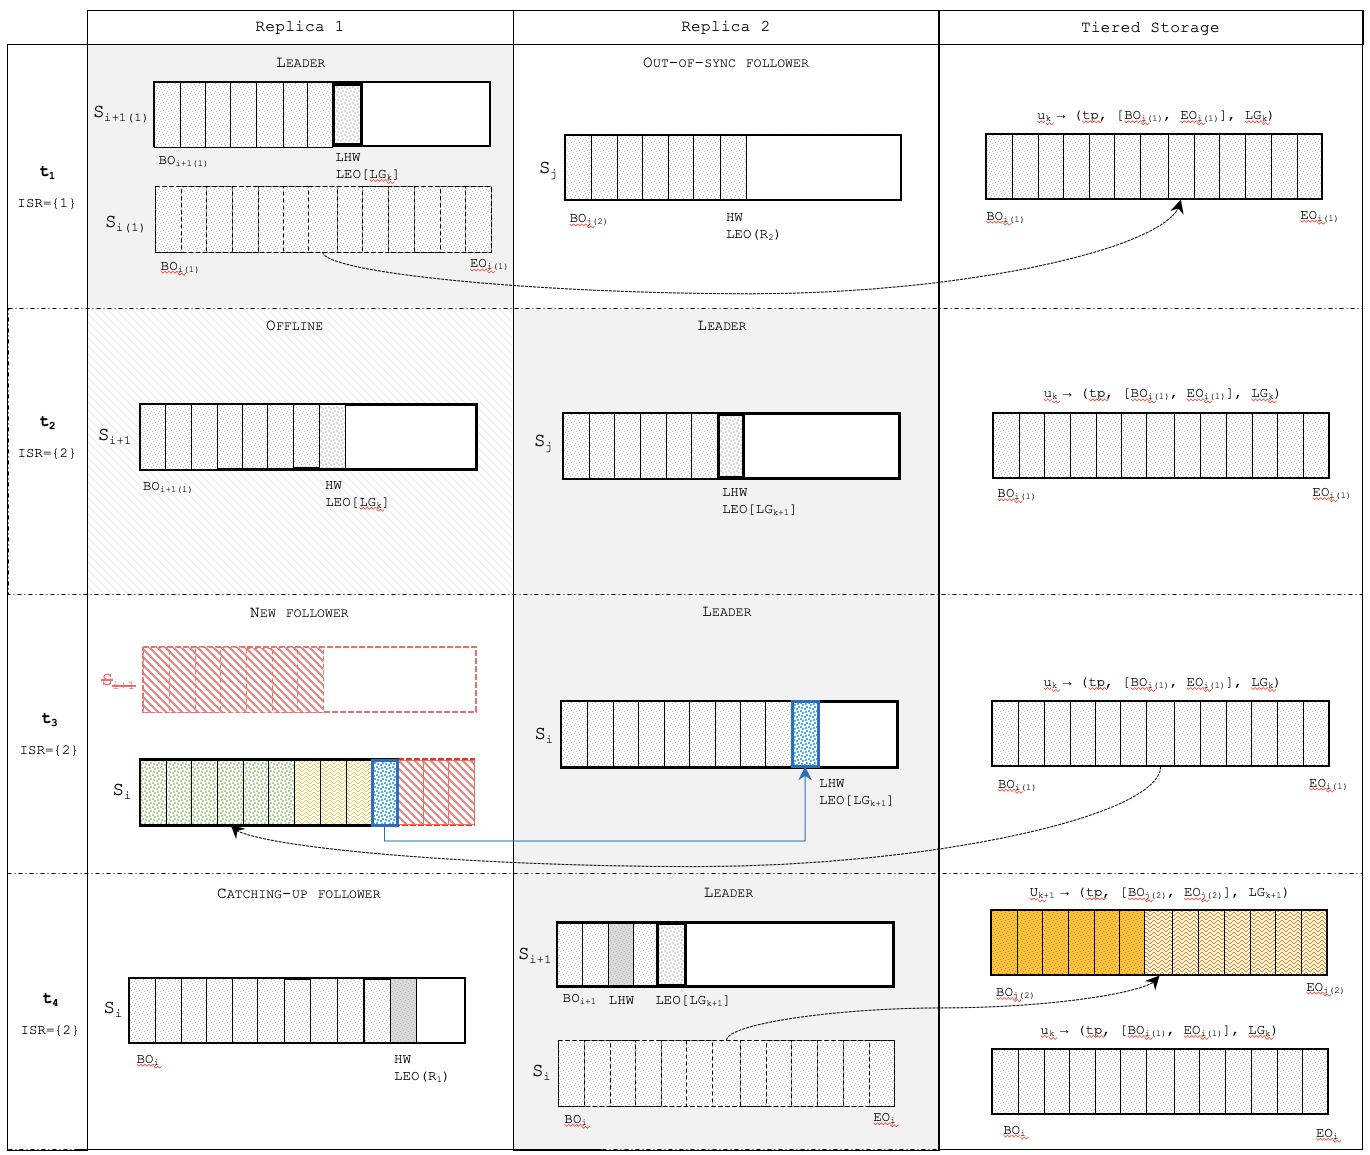
\includegraphics[scale=0.4]{unclean1.png}
	\captionof{figure}{Use of tiered segments to preserve local replica lineage.}
\end{center}

Shoud the segments $S(u_k)$ and $S(u_{k+1})$ be reconciled or deleted? 

Let us consider this follow-up use case, where a third replica is added to the previous example. This replica shares the same lineage as replica 1 up to generation $k$, then becomes offline at the same time as replica 1. It comes back online long after the latter, and replica 2 has produced segments $S_j^2$, $S_{j+1}^2$ and $S_{j+2}^2$. Assume $S_i^1$ is replicated by $S_i^3$ in replica 3, and that the latter is not available locally as it was deleted based on log retention policies. Replica 3 should follow the same replication steps as replica 1 to construct its lineage post-generation $k$.

The problem is segments $S_j^2$, $S_{j+1}^2$ and $S_{j+2}^2$ may be tiered and not available locally. That means that, to reconstruct its lineage, replica 3 would have to replicate segments from the tiered storage. One could argue that replica 3 could just replicate borrow the same lineage as replica 1 - but nothing guarantees lineage has not diverged after generation $k$ ! To illustrate this, imagine that before replica 3 is back online, replica 2 goes offline and replica 1 takes back leadership, ingests some records beyond $LEO_{k+1}$, then goes offline again, then replica 2 comes back and re-acquire leadership and resume ingesting. To preserve iso-functionality with local log segments, replica 3 needs to follow the exact same replication step to construct its lineage - and in the previous example, once replica 3 catches up with replica 2, lineages or replica 1 and 3 have diverged !

Note that evicting segments from the tiered storage for any of the replica \textit{lineage} could lead to catastrophic data loss. Consider the scenario where a topic-partition has three replicas, one of which has been offline for a month due to a misconfiguration. During a maintenance operation, the two "healthy" partitions are put offline and the "invalid" partition brought back online, empty. Unclean leader election is enabled and therefore the partition becomes leader. The one-month worth of data of the "healthy" replicas should be preserved, regardless of how many offsets and remote segments overlap with the new replica.

To allow tiered storage to preserve the durability guarantees of Apache Kafka, even under unclean leader election, all replica lineages would need to be kept.

\section{Objectives}


\end{document}
